\section{Lernfeld 6 - Datenbanken}

Im Lernfeld 6 werden neben Themen wie HTML, PHP und C# auch Datenbanken behandelt. Im Bereich der Datenbanken werden drei Begriffe unterschieden: (1) Datenbanken (DB), (2) Datenbankensystem (DBS) und (3) Datenbankmanagmentsystem (DBMS). Die folgende Grafik veranschaulicht den Zusammenhang.

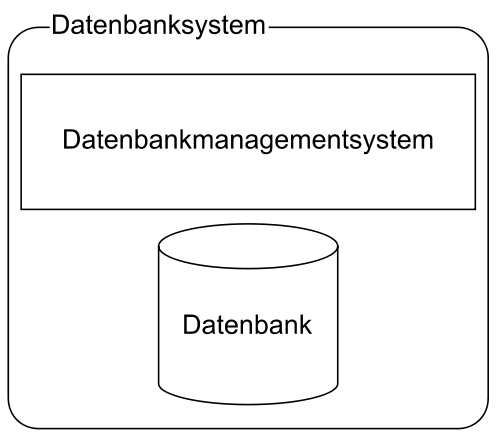
\includegraphics[scale=0.4]{pictures/lf06-pic/lf06-begriffszusammenhang.png}

Als DBS wird die Verbindung aus DBMS und der dazugehörigen Datenbank bezeichnet. Das DBMS regelt den Zugriff auf die Datenbank, sodass die Daten -- im besten Fall -- immer konsistent sind. 

\subsection{Datenbankenmodelle}

\subsubsection{Hierarchisches Datenbankmodell}
\subsubsection{Relationales Datenbankmodell}
\subsubsection{Netzwerkdatenbankmodell}
\subsubsection{Objektorientiertes Datenbankmodell}
\subsubsection{Objektrationales Datenbankmodell}


%%% MySQL
\subsection{MySQL}

Bei SQL handelt es sich um einen Standard zur Abfrage von Datenbanken. SQL wird unterteilt in vier Gebiete: (1) Data Definition Language, (2) Data Manipulation Language, (3) Data Query Language und (4) Data Conrol Language. In den folgenden Abschnitten werden die einzelnen Gebiete und deren Befehle anhand von Beispielen erklärt.

Umfassende Informationen zu den verschiedenen Befehlen lassen sich im Manual unter \url{http://dev.mysql.com/doc/refman/5.6/en/index.html} nachlesen.

\subsubsection{DDL -- Data Definition Language}
Beispiele für DDL-Befehle:

	\begin{itemize}
		\item source /path/to/geo.sql;
		\item drop table;
		\item alter
		\item create
	\end{itemize}

\subsubsection{DML -- Data Manipulation Language}
	
	\begin{itemize}
		\item delete 
		\item insert 
		\item update
	\end{itemize}
	
\subsubsection{DQL -- Data Query Language}
Enthält nur den Befehlt \ql select\qr. Diesem sind so viele Optionen zugeordnet, dass für ihn die eigene Kategorie \ql DQL\qr\ vorgesehen ist.

\subsubsection{DCL -- Data Conrol Language}
	
	\begin{itemize}
		\item grant
		\item revoke
	\end{itemize}
	
\subsubsection{Wildcards}

\begin{itemize}
	\item [\%]: beliebige Zeichen
	\item [\_]: für genau ein Zeichen
	\item [a-c]\%: Zeichenkette, die mit a,b oder c beginnt  
	\item [!a-c]\%: Zeichenkette, die \emph{nicht} a,b oder c beginnt
\end{itemize}

select * from fluss where name like "M\_k\%";
\begin{lstlisting}
#Beispielausgabe
+-----+---------+-----------------------+--------+
| FNR | Name    | Meer                  | Laenge |
+-----+---------+-----------------------+--------+
| MEK | Mekong  | Suedchinesisches Meer | 4500   |
| MSC | Mokscha | NULL                  | 656    |
+-----+---------+-----------------------+--------+
\end{lstlisting}

Wildcards beziehen sich nur auf Tabelleninhalte und nicht auf ihre Struktur
Unterschied zwischen \ql like\qr\ und \ql =\qr\ :
- \ql like\qr\ beherrscht Wildcards
- \ql =\qr\ kennt keine Wildcards, sondern interpretiert die Eingabe als String
- (- IS hat damit nichts zu tun; mit IS kann man keine Werte abfragen)

\subsubsection{Weitere Befehle}
\begin{itemize}
	\item show databases;
	\begin{lstlisting}
mysql> show databases;
+--------------------+
| Database           |
+--------------------+
| information_schema |
| geo                |
| mysql              |
| performance_schema |
+--------------------+
	\end{lstlisting}
	\item show tables;
	\begin{lstlisting}
mysql> show tables;
+---------------+
| Tables_in_geo |
+---------------+
| fluss         |
| kontinent     |
| land          |
| ort           |
| stadtfluss    |
+---------------+
	\end{lstlisting}
	\item 
	\item 
	\item 
\end{itemize}